\documentclass[12pt,letterpaper]{article}
\usepackage[frenchb]{babel}
\usepackage[margin=0.75in]{geometry}
\usepackage{hhline}
\usepackage{graphicx}
\graphicspath{ {images/} }

\title{Eclipse X - BMS}
\author{
	Daigneault-St-Arnaud, Christian, DAIC30099006
}
\newcommand{\cours}{ }
\newcommand{\prof}{ }


\begin{document}
	
	\begin{titlepage}
	\makeatletter
		\pagenumbering{gobble}
		\centering
		\vspace{5cm}
		{\Huge \@title}\\ 
		\vspace{5cm}
		{\large 
			Par \\
			\vspace{0.5cm}
			\@author \\
			\vspace{5cm}
			%\cours \\
			%\vspace{0.5cm}
			%\prof \\
			%\vspace{3.5cm}
			\@date \\
			\vspace{5cm}
			\'{E}COLE DE TECHNOLOGIE SUP\'{E}RIEURE \\
			UNIVERSIT\'{E} DU QUÉBEC
		}
		\newpage
	\end{titlepage}
	\tableofcontents
	\newpage
	\pagenumbering{arabic}
	\begin{normalsize}
		\section{Lecture de tension des modules}
			\subsection{Objectifs}
				Nous d\'{e}sirons avoir une lecture tr\`{e}s pr\'{e}sise (+/- 2mV) du modules. Afin de pouvoir brancher les modules dans n'importe quel ordre sur le BMS, nous devons faire en sorte que les lectures de tension sont isol\'{e}es.Le circuit doit consommer un minimum de courant puisqu'il sera aliment\'{e} par le modules.
			\subsection{Circuit analogique}
				\subsubsection{Sch\'{e}ma}
				\begin{center}
					% Schema
					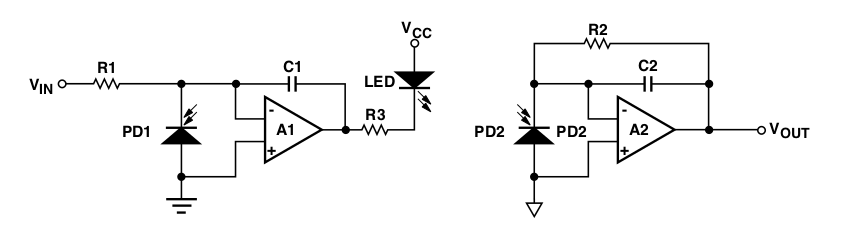
\includegraphics[scale=0.5]{Analog} \\ \vspace{1cm}
				\end{center}
			
				\subsubsection{Analyse}
				\begin{center}
					
					%  BOM
					BOM \\ \vspace{0.25cm}
					\begin{tabular}{|c|c|c|}
						\hline
						Part number & Description & Prix (total)\\ \hhline{|=|=|=|}
						BU7421SG-TR & Op-amp (2x) & 2\$ \\ \hline
						LOC110STR & Optocoupleur lin\'{e}aire & 4.09\$ \\ \hline
						 \multicolumn{2}{|c|}{ }& 6.09\$ \\ \hline
						 \multicolumn{3}{r}{ } Prix de digikey pour 1 unit\'{e} \\
					\end{tabular}\\ \vspace{0.5cm}
					% Fin BOM
				
					% Avantage // Desavantage
					Analyse de la solution \\ \vspace{0.25cm}
					\begin{tabular}{|c|c|}
						\hline
						Avantage & D\'{e}savantage\\ \hhline{|=|=|}
						Peut de composantes & Pr\'{e}cision de +/- 1\% \\ \hline
						Robuste & L'optocoupleur lin\'{e}aire est gros (SOIC 8)\\ \hline
						 & Consomme beaucoup de courant (10mA max)\\ \hline
					\end{tabular} \\ \vspace{0.5cm}
					% Fin Avantage // Desavantage
				\end{center} 
				\subsubsection{Conclusion}
				% Conclusion
				Le circuit analogique autour de l'optocoupleur lin\'{e}aire n'est pas assez pr\'{e}cis pour \^{e}tre consid\'{e}r\'{e} comme viable pour le projet.De plus, il consomme beaucoup trop de courant pour pouvoir \^{e}tre toujours en marche. Il faudrait ajouter un circuit pour d\'{e}sactiver la lecture lorsqu'elle n'est pas utilis\'{e}. Ceci enl\`{e}ve l'avantage d'utiliser cette solution. 
				\newpage
				
			\subsection{Circuit digital}
				\subsubsection{Protocole de communication}
					Les ADC externes utilisent souvent les m\^{e}me trois interface de communication s\'{e}riel : UART,I2C et SPI. Puisque nous avons un nombre limit\'{e} de ces periph\'{e}rique sur le microcontr\^{o}leur, nous aurons besoin d'un bus qui permet d'avoir un maximum d'ADC. Il nous reste donc le choix entre le I2C et le SPI. Le SPI demanderais d'avoir un circuit d'isolation consid\'{e}rablement plus gros et dispendieux que le I2C. Le SPI \`{a} deux fils de plus que le I2C ( 1 pour le data et 1 pour choisir le "slave"). \\
					Le protocol choisis est le I2C et le circuit d'isolation est le ISO1541DR. Malheureusement, le circuit consomme un petit peu moins de 5mA. Nous devrons donc avoir une alimentation qui permettra de d\'{e}sactiver l'alimentation du c\^{o}t\'{e} du modules lorsque le syst\`{e}me ne sera pas en marche.
					
				\subsubsection{Lecture d'un voltage de reference}
					
				
				\subsubsection{Lecture du voltage de la cellule}
					MCP3221A5T => Non adressable
					ADC121C021CIMM/NOPB
				
	\end{normalsize}
\end{document}
\makeatother


